\documentclass[10pt]{beamer}
\usepackage{lmodern}
\usepackage{amssymb}
\usepackage{graphicx}
\usepackage{amsmath}
\usepackage{multirow}
\usepackage{mathtools}
\usepackage{placeins}
\usepackage{lscape}
\usepackage{geometry}
\usepackage{dcolumn}
\usepackage[utf8]{inputenc}
\usepackage{hyperref}
\usepackage{tabularx}
\usepackage{nicematrix}
\usepackage{calc}
\usepackage{qtree}
\usepackage{tikz}
\usetikzlibrary{shapes.geometric, arrows}

\usetheme{Boadilla}


\title{SOFR so good? New Benchmark Rate and Crowding-Out Effect}  
\author{Qian Wu}
\date{\today} 

\makeatletter
\newcommand\MyInfo[1]{%
\setbeamertemplate{footline}
{
  \leavevmode%
  \hbox{%
  \begin{beamercolorbox}[wd=.22\paperwidth,ht=2.25ex,dp=1ex,center]{author in head/foot}%
    \usebeamerfont{author in head/foot}#1
  \end{beamercolorbox}%
  \begin{beamercolorbox}[wd=.56\paperwidth,ht=2.25ex,dp=1ex,center]{title in head/foot}%
    \usebeamerfont{title in head/foot}\insertshorttitle
      \end{beamercolorbox}%
  \begin{beamercolorbox}[wd=.22\paperwidth,ht=2.25ex,dp=1ex,right]{date in head/foot}%
    \usebeamerfont{date in head/foot}\insertshortdate{}\hspace*{2em}
    \insertframenumber{} / \inserttotalframenumber\hspace*{2ex} 
  \end{beamercolorbox}}%
  \vskip0pt%
}
}
\makeatother

\tikzstyle{io} = [rectangle, rounded corners, minimum width=3cm, minimum height=.7cm,text centered, draw=black, fill=blue!30]
\tikzstyle{arrow} = [thick,->,>=stealth]


\begin{document}
\MyInfo{Qian Wu}


\begin{frame}
\titlepage
\end{frame} 


\begin{frame}
\frametitle{Background Info}
\begin{itemize}
\item LIBOR is the reference interest rate used worldwide in a large variety of financial assets including business loans,  consumer loans,  and derivatives.
\item Due to the LIBOR manipulation scandal and a shrinking interbank debt market,  LIBOR is being retired.  In the US,  the Alternative Reference Rate Committee (ARRC) recommends SOFR as the alternative to the USD LIBOR.
\item \textbf{LIBOR}: London Interbank Offered Rate
\begin{itemize}
\item LIBOR is the average interest rate that leading banks borrow from each other. 
\item  It's based on banks' own estimation,  not real transactions.
\item It reflects banks' borrowing cost,  thus includes banks credit premium.
\end{itemize}
\item \textbf{SOFR}: Secured Overnight Financing Rate
\begin{itemize}
\item SOFR is a broad measure of the cost of borrowing cash overnight collateralized by Treasury securities.
\item It's based on the real transactions in the overnight Treasury repurchase market.
\item It's nearly risk-free.
\end{itemize}
\end{itemize}
\end{frame}


\begin{frame}
\frametitle{SOFR and LIBOR}
\begin{center}
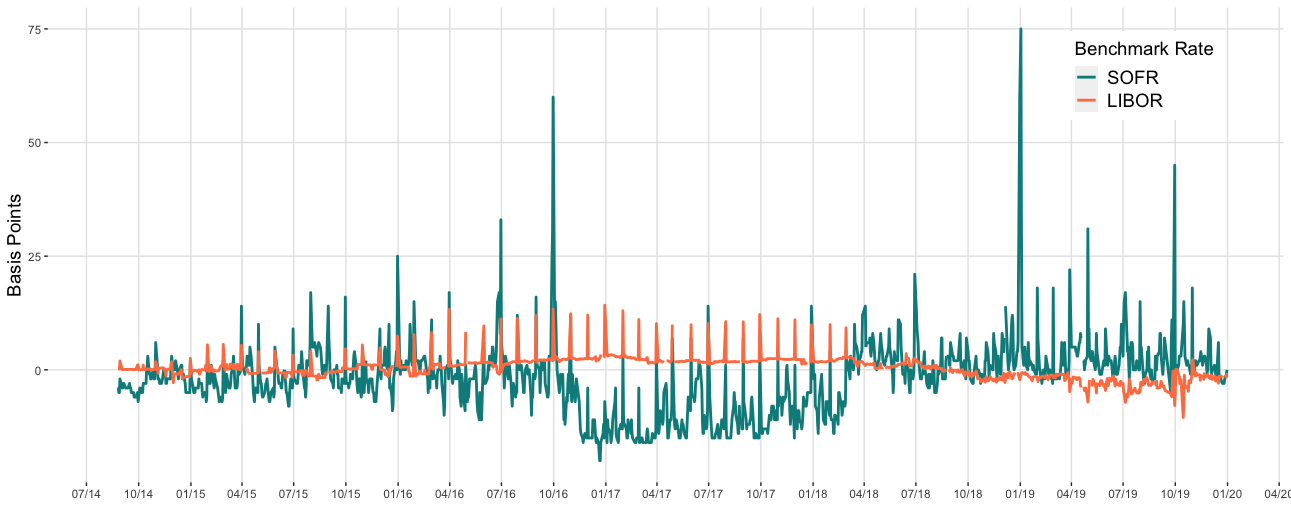
\includegraphics[scale=.25]{rates.png}\\
\tiny Fig 1: Spread of SOFR and LIBOR over FFR
\end{center}
\end{frame}


\begin{frame}
\frametitle{Research Question}
Does the change of the benchmark interest rate affect the size of the government debt crowding out effect?
\begin{itemize}
\item \textbf{Crowding-Out Effect}: Gov't issues more Treasuries $\rightarrow$ Demand for loanable funds increases $\rightarrow$ Interest rate increases $\rightarrow$ Private spending decreases
\item Since SOFR is based on transactions collateralized by Treasuries,  the economy with SOFR may obtain a larger magnitude of crowding-out effect.
\end{itemize}
\end{frame}

\begin{frame}
\frametitle{Literature Review}
Since the transition from LIBOR to SOFR is still ongoing \footnote{The publication for one-week and two-month USD LIBOR will cease on December 31, 2021; The publication for the USD LIBOR with other terms will cease on June 30, 2023.},  there has been limited literature studying the implications of switching benchmark rate.
\begin{itemize}
\item Klingler and Syrstad (2021) empirically examine SOFR,  SONIA,  and ESTR.  They identify three drivers of alternative benchmarks: regulatory constraints,  \textcolor{blue}{government debt},  and central bank reserves.
\item Jermann (2019) uses a quantitative model to show that,  when banks have an increased funding cost risk,  LIBOR offer insurance while SOFR does not.  Therefore,  in a SOFR economy banks default more and firms reduce investment more.
\end{itemize}
\end{frame}


\begin{frame}
\frametitle{Collateral Channel}
\begin{itemize}
\item In economy with SOFR,  the crowding-out effect can be amplified through the following channel:
\begin{itemize}
\item Gov't issues Treasuries $\xrightarrow {\text{link1}}$ Treasury holders finance on Treasury Repo market,  thus demand for collateralized borrowing increases $\xrightarrow {\text{link2}}$ SOFR rises $\xrightarrow {\text{link3}}$ Business loans become more costly $\xrightarrow{\text{link4}}$ Investment decreases
\end{itemize}
\item Possible Flaws:
\begin{itemize}
\item link 1: Treasury buyers may not engage in Repo market financing activity.
\item link 2: SOFR may not rise if the demand for reverse Treasury Repo rises.
\item link 3: Will the majority of business loans be indexed by SOFR?
\item link 4: Firms may alternatively finance using equity or corporate bonds.
\end{itemize}
\end{itemize}
\end{frame}


\begin{frame}
\frametitle{Empirical Evidence}
\begin{itemize}
\item Gov't issues Treasuries $\xrightarrow {\text{link1}}$ Treasury holders finance on Treasury Repo market,  thus demand for collateralized borrowing increases $\xrightarrow {\text{link2}}$ SOFR rises $\xrightarrow {\text{link3}}$ Business loans become more costly $\xrightarrow{\text{link4}}$ Investment decreases
\item To concrete the logic chain,  several empirical evidences are investigated.
\begin{itemize}
\item link 1: Regression shows that Treasury Repo transaction made by primary dealers increases with government debt.
\item link 1 + 2: Regression shows that SOFR increases with government debt.
\item link 3: Leading financial institutions indicated that they are ready to use SOFR for business loans.
\item link 4: Business loan is a significant component of firms' total debt.
\end{itemize}
\end{itemize}
\end{frame}


\begin{frame}
\frametitle{Treasury Repo and Gov't Debt (link 1)}
\begin{itemize}
\item Primary dealers purchase over 70\% of Treasury securities sold to the public.\\
\vspace{3mm}
\begin{center}
{\footnotesize%
\begin{tabular}{lcccc} 
\multicolumn{5}{c}{Table 1: Bidder Category Purchase Shares for Treasury Securities}\\\hline
Category & Mean & Std & Minimum & Maximum \\ \hline
 &  &  &  &  \\
\textcolor{blue}{Primary dealer} & 70.9 & 14.6 & 33.6 & 100 \\
Direct bidder & 2.4 & 3.6 & 0.0 & 31.6 \\
Indirect bidder & 21.6 & 12.7 & 0.0 & 64.8 \\
Noncompetitive & 5.1 & 4.7 & 0.0 & 16.8 \\ \hline
\multicolumn{5}{l}{ Source: Fleming, M. J. (2007). Who buys Treasury securities at auction?} \\
\multicolumn{5}{l}{Note: The calculation is based on 576 US Treasury auctions between May 5, 2003, }\\
\multicolumn{5}{l}{\hspace{7mm} and December 28, 2005.}
\end{tabular}
}%
\end{center}
\end{itemize}
\end{frame}


\begin{frame}
\frametitle{Treasury Repo and Gov't Debt (link 1),  Cont'd}
\begin{itemize}
\item Focusing on primary dealers,  I regress their Treasury Repo volumes on government debt outstanding.
\begin{center}
  {\scriptsize%
\begin{tabular}{@{\extracolsep{1pt}}lD{.}{.}{-3} D{.}{.}{-3} } 
\multicolumn{3}{c}{Table 2: Response of primary dealers' Repo Activity to Government Debt Issuance}\\[1ex]\hline 
\hline \\[-1.8ex] 
 & \multicolumn{2}{c}{\textit{Dependent variable:}} \\ 
\cline{2-3} 
\\[-1.8ex] & \multicolumn{2}{c}{Primary dealers' Repo} \\ 
\\[-1.8ex] & \multicolumn{1}{c}{(1)} & \multicolumn{1}{c}{(2)}\\ 
\hline \\[-1.8ex] 
 Government debt & 1.465^{**} & 1.073^{*} \\ 
  & (0.590) & (0.549) \\ 
  Lagged Repo &  & -0.245^{***} \\ 
  &  & (0.051) \\ 
  Constant & -0.001 & -0.0004 \\ 
  & (0.001) & (0.001) \\ 
 \hline \\[-1.8ex] 
Adjusted $R^2$ & 0.0197 & 0.0756 \\ 
Observations & 351 & 350 \\ 
\hline 
\hline \\[-1.8ex] 
\multicolumn{3}{l}{Note: $^{*}$p$<$0.1; $^{**}$p$<$0.05; $^{***}$p$<$0.01} \\ 
\multicolumn{3}{l}{\hspace{7mm}All variables are in diff log format.}\\
\multicolumn{3}{l}{\hspace{7mm}Newey-West Standard Error in parenthesis.}\\
\multicolumn{3}{l}{\hspace{7mm}The sample includes weekly data from January 7, 2015 to November 3, 2021.}
\end{tabular} 
}%
\end{center}
\item The result shows that primary dealers participate more in the Treasury Repo market after government debt issuance.
\end{itemize}
\end{frame}


\begin{frame}
\frametitle{Response of SOFR to Gov't Debt (link 1+2)}
\begin{itemize}
\item To show that SOFR is more sensitive to Treasury issuance than LIBOR,  I regress both SOFR and LIBOR on government debt outstanding.
\begin{center}
  {\scriptsize%
\begin{tabular}{@{\extracolsep{1pt}}lD{.}{.}{-3} D{.}{.}{-3} D{.}{.}{-3} D{.}{.}{-3} } 
\multicolumn{5}{c}{Table 3: Response of SOFR and LIBOR to Government Debt Issuance}\\[.8ex]\hline 
\hline \\[-1.8ex] 
 & \multicolumn{4}{c}{\textit{Dependent variable:}} \\ 
\cline{2-5} 
\\[-1.8ex] & \multicolumn{2}{c}{SOFR} & \multicolumn{2}{c}{LIBOR} \\ 
\\[-1.8ex] & \multicolumn{1}{c}{(1)} & \multicolumn{1}{c}{(2)} & \multicolumn{1}{c}{(3)} & \multicolumn{1}{c}{(4)}\\ 
\hline \\[-1.8ex] 
Government debt & 614.474^{***} & 609.553^{***} & -36.676 & -34.162 \\ 
  & (166.458) & (169.146) & (23.319) & (22.558) \\ 
  Lagged SOFR &  & 0.173^{**} &  &  \\ 
  &  & (0.078) &  &  \\ 
  Lagged LIBOR &  &  &  & -0.163^{**} \\ 
  &  &  &  & (0.066) \\ 
  Constant & -0.276^{***} & -0.242^{***} & 0.008 & 0.008 \\ 
  & (0.088) & (0.068) & (0.010) & (0.011) \\ 
 \hline \\[-1.8ex] 
Adjusted $R^2$ & 0.0405 & 0.0696 & 0.0026 & 0.0283 \\ 
Observations & 1135 & 1134 & 1100 & 1082 \\ 
 \hline \\[-1.8ex] 
\hline 
 \multicolumn{5}{l}{Note: $^{*}$p$<$0.1; $^{**}$p$<$0.05; $^{***}$p$<$0.01} \\ 
 \multicolumn{5}{l}{\hspace{7mm}All variables are in diff log format.}\\
\multicolumn{5}{l}{\hspace{7mm}Newey-West Standard Error in parenthesis.}\\
\multicolumn{5}{l}{\hspace{7mm}The sample includes daily data from August 25, 2014 to December 31, 2019.}
\end{tabular} 
}%
\end{center}
\item The results show that issuing government debt is correlated with higher SOFR level while it has no significant effect on LIBOR.
\end{itemize}
\end{frame}


\begin{frame}
\frametitle{Business Loans Picking up SOFR (link 3)}
A considerable share of business loans will be indexed by SOFR because (1) there exists a large scale of floating-rate business loans indexed by LIBOR; (2) leading banks indicate they will pick up SOFR after LIBOR retires.
\begin{itemize}
\item Among cash products, business loans have the highest exposure to USD LIBOR. 
\begin{center}
{\footnotesize%
\begin{tabular}{lccccc}
\multicolumn{6}{c}{Table 4: Estimated Business Loans Exposed to USD LIBOR}\\\hline
 &Volume  & \multicolumn{4}{c}{Share Maturing By:}\\ 
 &(Trillions USD)  &2021 & 2025  &2030 & 2040 \\ \hline
 Syndicated loans & 1.5 & 83\% & 100\% & 0\% & 0\% \\
 Nonsyndicated loans & 0.8 & 86\% & 97\% & 1\% & 0\% \\
 Commercial mortgages & 1.1 & 83\% & 94\% & 4\% & 2\% \\
 \hline \hline
\multicolumn{6}{l}{ Source: Second Report of The Alternative Reference Rates Committee.} \\
\multicolumn{6}{l}{Note: Data are gross national exposures as of year-end 2016.  }\\
\multicolumn{6}{l}{\hspace{7mm} At of year-end 2016,  total national nonfinancial business nonmortgage loan is } \\ 
\multicolumn{6}{l}{\hspace{7mm} 4.1(?) trillions of USD and total commercial mortgage is 4.2(?) trillions of USD. }
\end{tabular}
}%
\end{center}
\end{itemize}
\end{frame}


\begin{frame}
\frametitle{Business Loans Picking up SOFR (link 3),  Cont'd}
\begin{itemize}
\item Leading banks have explicitly or implicitly indicated that they will pick up SOFR as the replacement for LIBOR.
\begin{itemize}
\item \textbf{JPMorgan Chase}: All new loan financings, such as for mergers and acquisitions that JPMorgan is underwriting are being tied to SOFR if they are expected to price next year, said Kevin Foley, the bank's global head of capital markets. (Financial Times)
\item \textbf{BOA}: Grabenstein added Wells Fargo has not "put a total stop on LIBOR loans, but we are going to the customer with SOFR first and only if there is a real need to use LIBOR should it still be considered." (Financial Times)
\item \textbf{U.S.  Bank}: U.S. Bank became operationally ready to offer SOFR for most commercial loans.  (U.S.Bank website)
\item \textbf{Truist}: At Truist we offer SOFR as an alternative rate for commercial loans...(Truist website)
\item \textbf{TD Bank}: For LIBOR indexed loans with tenors after the anticipated phase-out date, we plan to offer three SOFR varieties based on customer preference or appropriateness as alternatives to LIBOR after the phase-out date.  (TD Bank website)
\end{itemize}
\end{itemize}
\end{frame}


\begin{frame}
\frametitle{\large Business Loans in Total Debt of Nonfinancial Sectors (link 4)}
\begin{center}
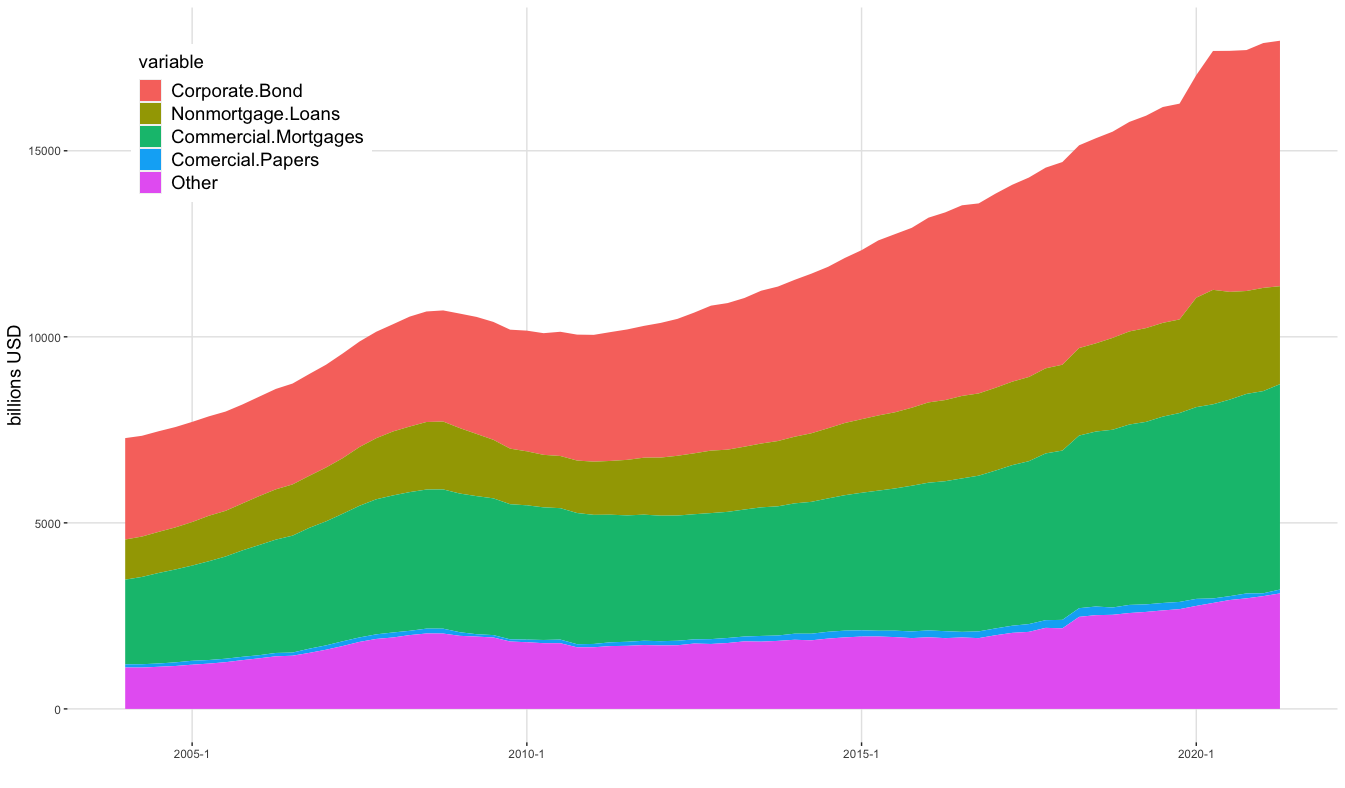
\includegraphics[scale=.22]{businessdebt.png}\\
\tiny Fig 2: Components of National Business Debts
\end{center}
\end{frame}


\begin{frame}
\frametitle{Next Steps}
\begin{itemize}
\item More robust empirical evidences; Causal inference
\item Quantitative model
\end{itemize}
\end{frame}



\begin{frame}
  \frametitle{Local Projection}
Two Steps:
\begin{itemize}
  \item Compute borrowing shocks
  \begin{align*}
    b_t=\alpha_0+\alpha_1t+\alpha_2t^2+A(L)X_{t-1}+\epsilon_t^b
  \end{align*}
  \begin{itemize}
    \item $b_t$: log(govt debt)
    \item $X_t$: controls including six lags of log(govt debt), log(industrial production), and log(stock price)
    \item $\hat{\epsilon}_t^b$: identified borrowing shock
  \end{itemize}
  \item Estimate local projections
  \begin{align*}
    r_{t+h}=\beta_0+\psi_h \hat{\epsilon}_t^b +\Gamma(L)Z_{t-1}+u_{t+h}
  \end{align*}
    \begin{itemize}
      \item $r_{t+h}$: SOFR or LIBOR spread at horizon h
      \item $Z_{t-1}$: controls including three lags of SOFR or LIBOR spread, log(govt debt), and log(industrial production)
    \end{itemize}
\end{itemize}
\end{frame}


\begin{frame}
  \frametitle{LP Results}
  \begin{center}
    IRFs of Government Borrowing Shock
    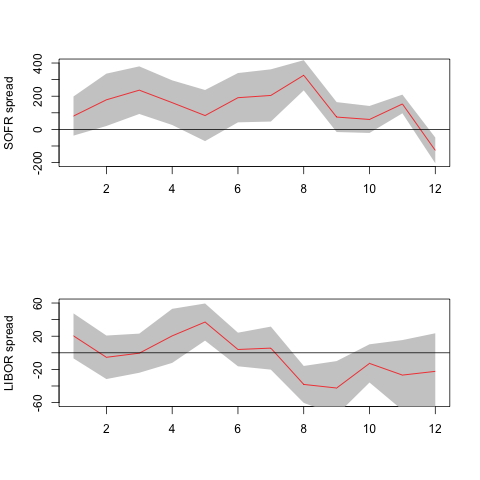
\includegraphics[scale=0.5]{irfs.png}
  \end{center}
\end{frame}



\end{document}

